% Section content template for individual Educative lessons
% This file contains the actual content for a specific section
% Generated from Educative API section content

% Section: Sequence Diagram
% Section ID: 5224098311700480
% Section Slug: sequence-diagram
% Generated: 2025-12-08T22:22:38.400693

A \textbf{sequence diagram} is a form of communication diagram that illustrates how different actors and objects interact with each other or between themselves. The diagram represents these interactions as an exchange of messages between various entities and the type of exchange. Sequence diagrams also demonstrate the sequence of events that occur in a specific use case and the logic behind different operations and functions.

\subsection{Elements of a sequence diagram}\label{elements-of-a-sequence-diagram}
\\
Various elements make up a sequence diagram. Let\textquotesingle s discuss some of the essential elements of this diagram that appear most often.

\subsubsection{Lifeline}\label{lifeline}
\\
In sequence diagrams, we write all entities horizontally. Each entity has a \textbf{lifeline} that represents its existence, i.e., when the entity is activated or deactivated. We illustrate this using a dotted line below the entity. We represent different objects, actors, entities, or boundaries in a system using lifelines, and they never overlap each other. The illustration below shows how to visualize a lifeline in UML. The horizontal boxes are used to denote the objects involved in the interaction.

\begin{figure}[htbp]
 \centering
 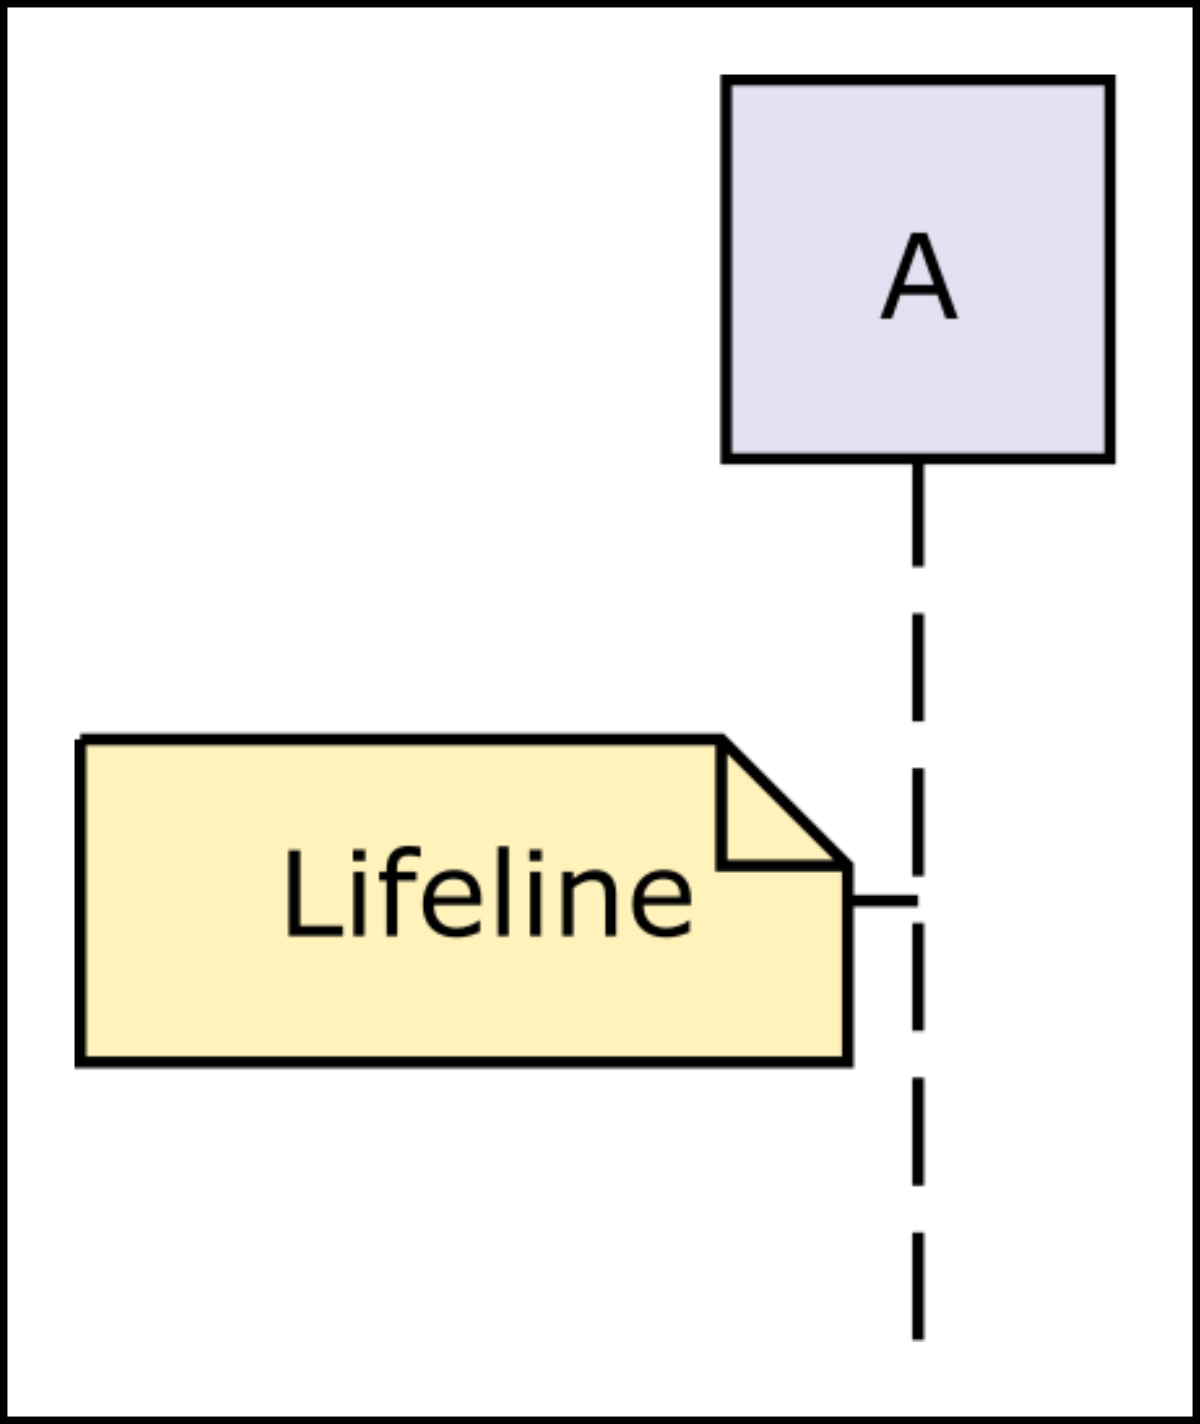
\includegraphics[width=0.25\textwidth]{Images/chapter_3/section_5224098311700480/4821997840498688.png}
 \caption{Lifeline in a sequence diagram}
\end{figure}

\subsubsection{Activation bars}\label{activation-bars}
\\
Activation bars indicate the \textbf{active period} of an object, that is, the time when an object sends or receives messages. We draw these using simple vertical boxes on the lifeline. Here\textquotesingle s an example of an activation bar:

\begin{figure}[htbp]
 \centering
 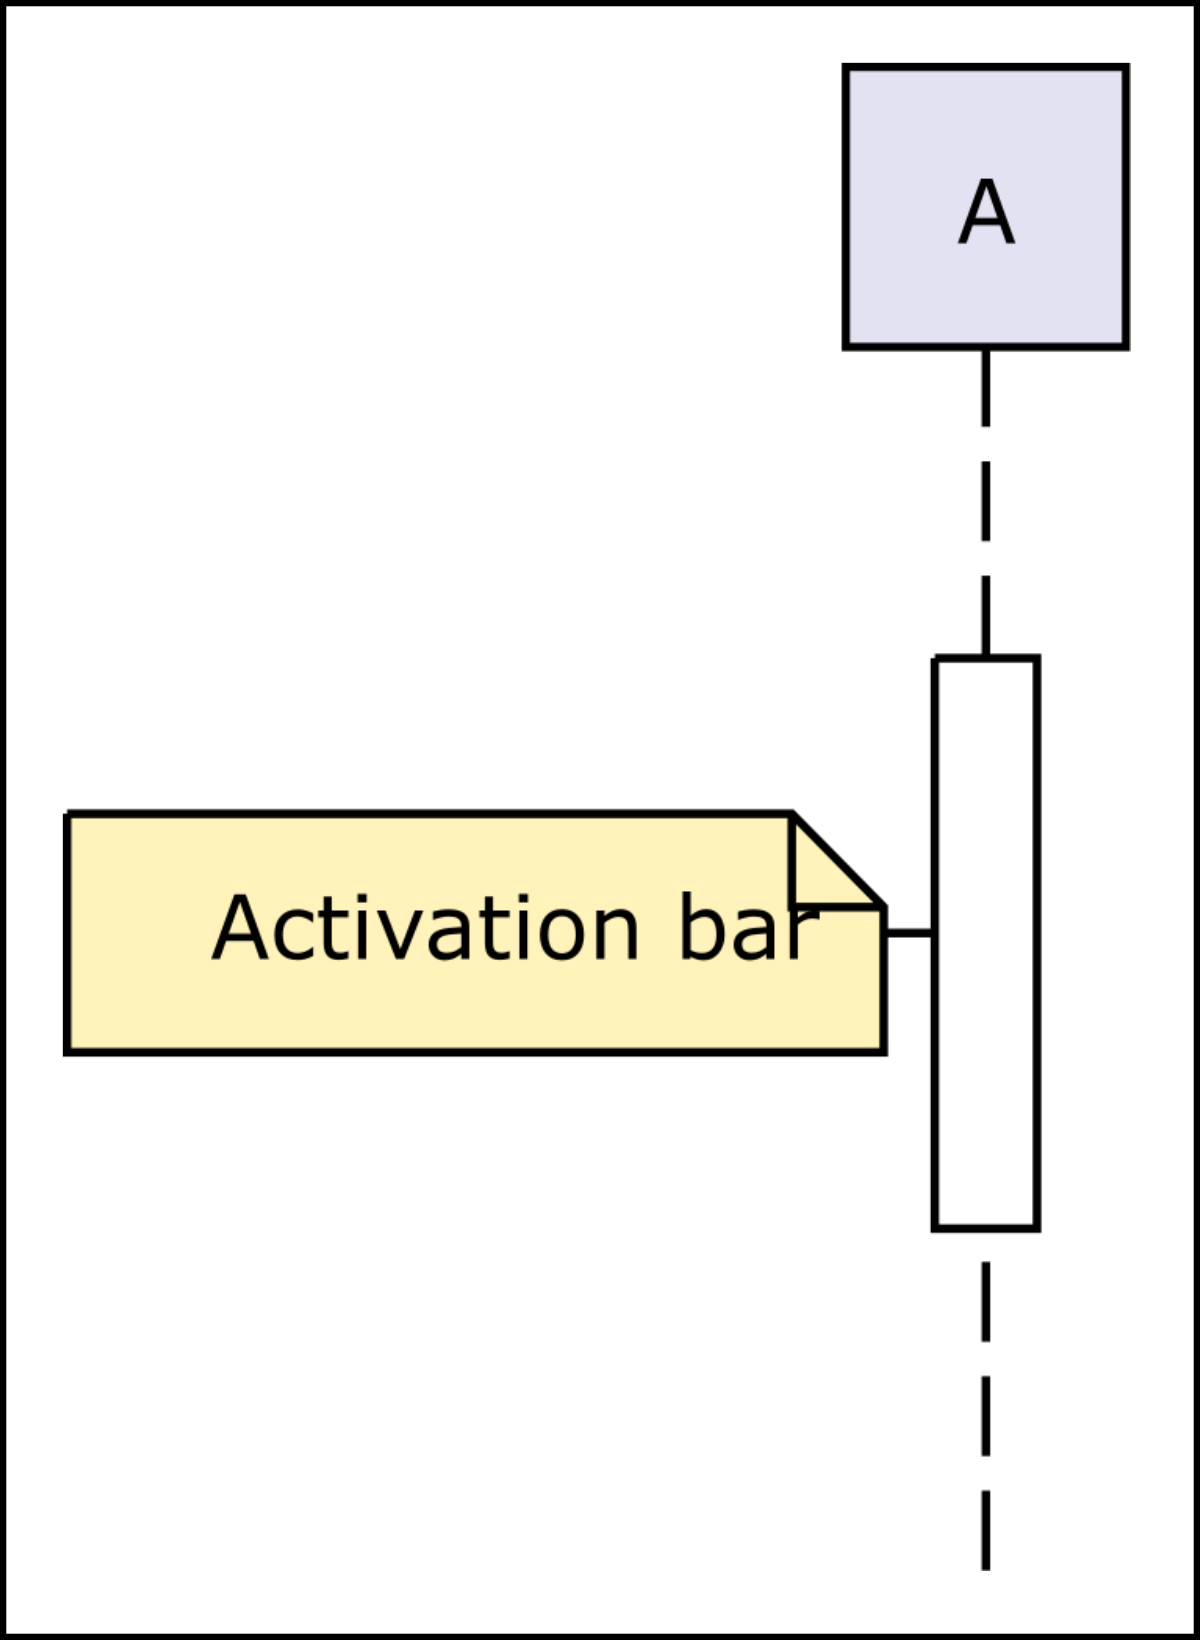
\includegraphics[width=0.25\textwidth]{Images/chapter_3/section_5224098311700480/6009898653712384.png}
 \caption{Activation bar in a sequence diagram}
\end{figure}

\subsubsection{Messages}\label{messages}
\\
In sequence diagrams, a message is an interaction between two objects. It can be in the form of sending and receiving messages, invoking an operation, or creating a new object or entity. Messages are drawn horizontally in any direction: left to right, right to left, or back to themselves. Different kinds of messages are represented using different arrows. Let\textquotesingle s look at the types of messages:

\begin{enumerate}
\item
A \textbf{synchronous message} is a type of message where the sender has to wait for the receiver to return a response before it can perform another operation. We can draw synchronous messages using a solid line with a filled arrowhead.
\end{enumerate}

\begin{figure}[htbp]
 \centering
 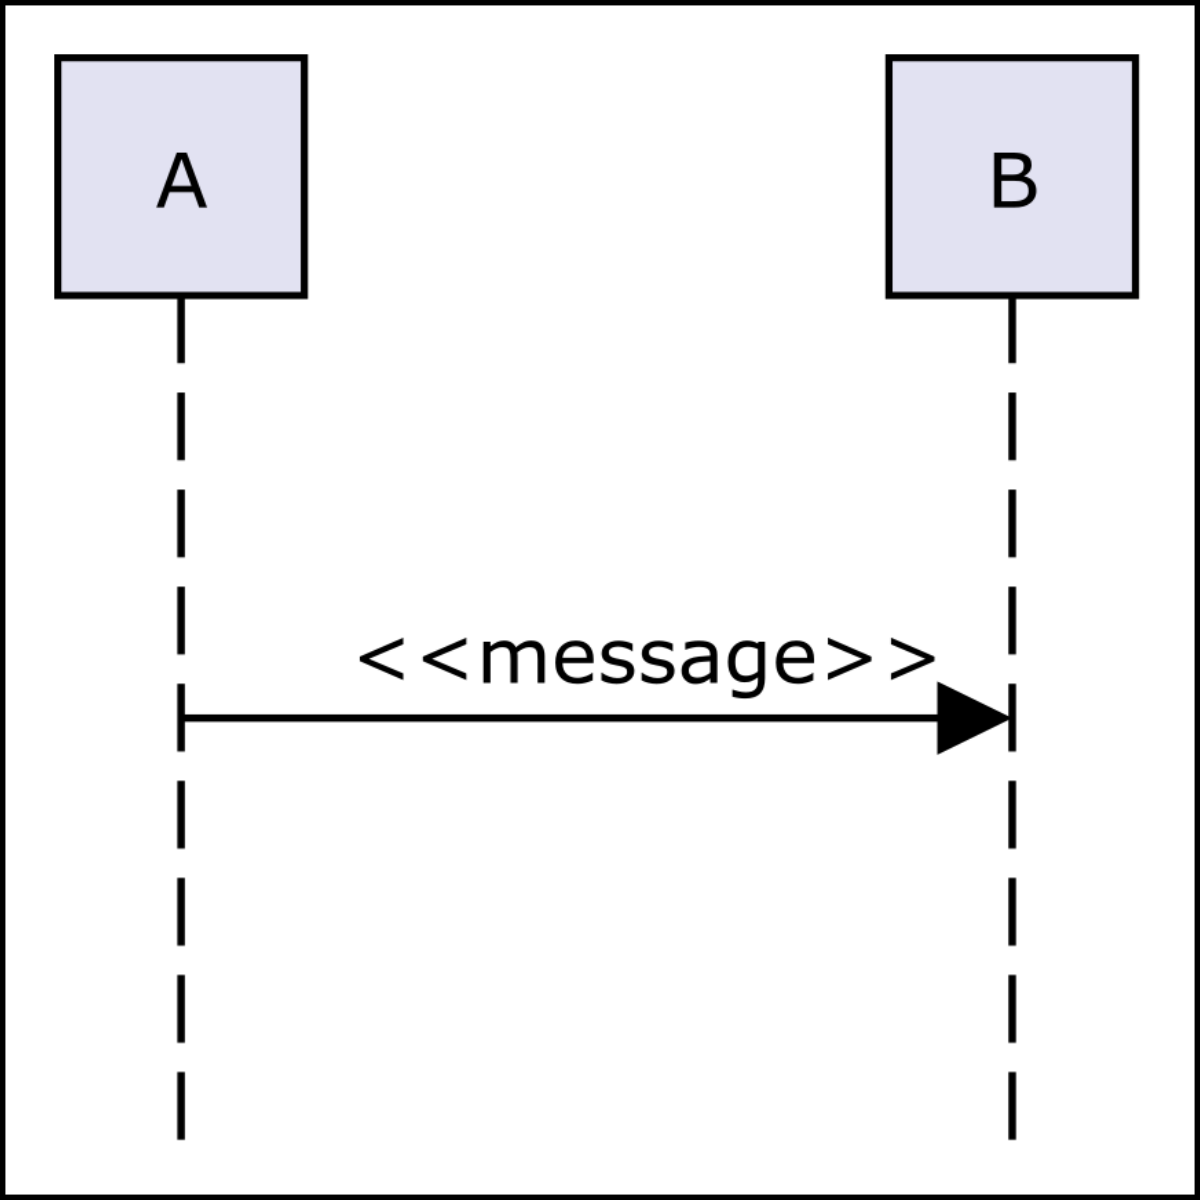
\includegraphics[width=0.25\textwidth]{Images/chapter_3/section_5224098311700480/5205443880419328.png}
 \caption{A synchronous message}
\end{figure}

\begin{enumerate}
\setcounter{enumi}{1}
\item
An \textbf{asynchronous message} is a type of message where the sender does not have to wait for a response from the receiver. The sender can continue sending messages to other objects. We can draw the asynchronous messages using a solid line with an open arrowhead.
\end{enumerate}

\begin{figure}[htbp]
 \centering
 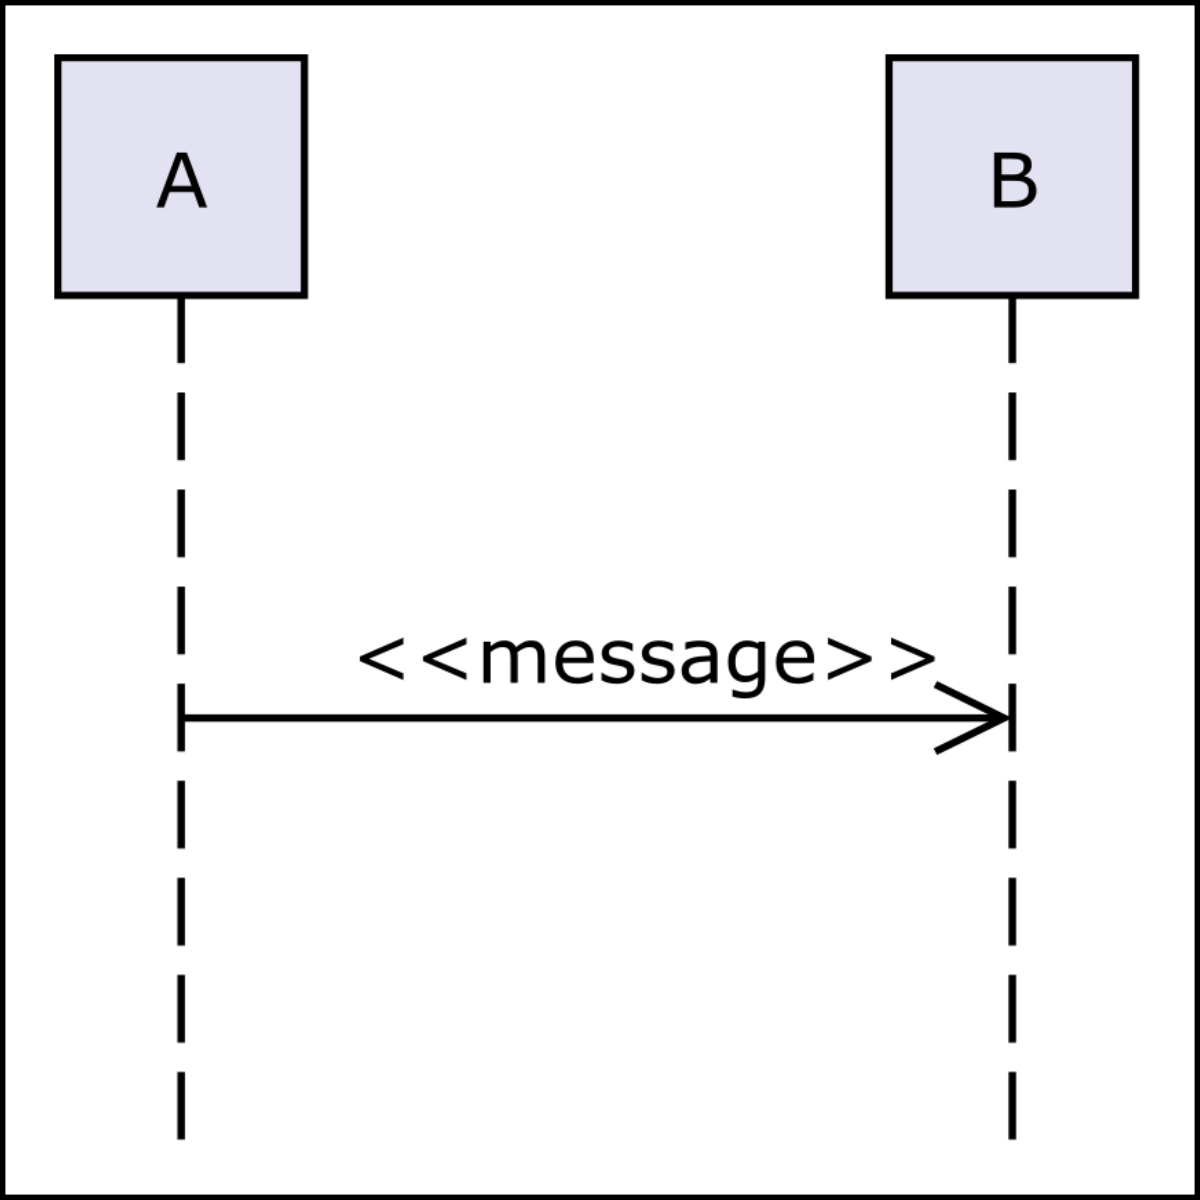
\includegraphics[width=0.25\textwidth]{Images/chapter_3/section_5224098311700480/6113614044069888.png}
 \caption{An asynchronous message}
\end{figure}

\begin{enumerate}
\setcounter{enumi}{2}
\item
A \textbf{synchronous return} is a type of message generated in response to a synchronous call. A synchronous message has to be paired with a synchronous return message. It means that the receiver has processed the message and sent a response. We can draw synchronous return messages using a dotted line with a filled arrowhead.
\end{enumerate}

\begin{figure}[htbp]
 \centering
 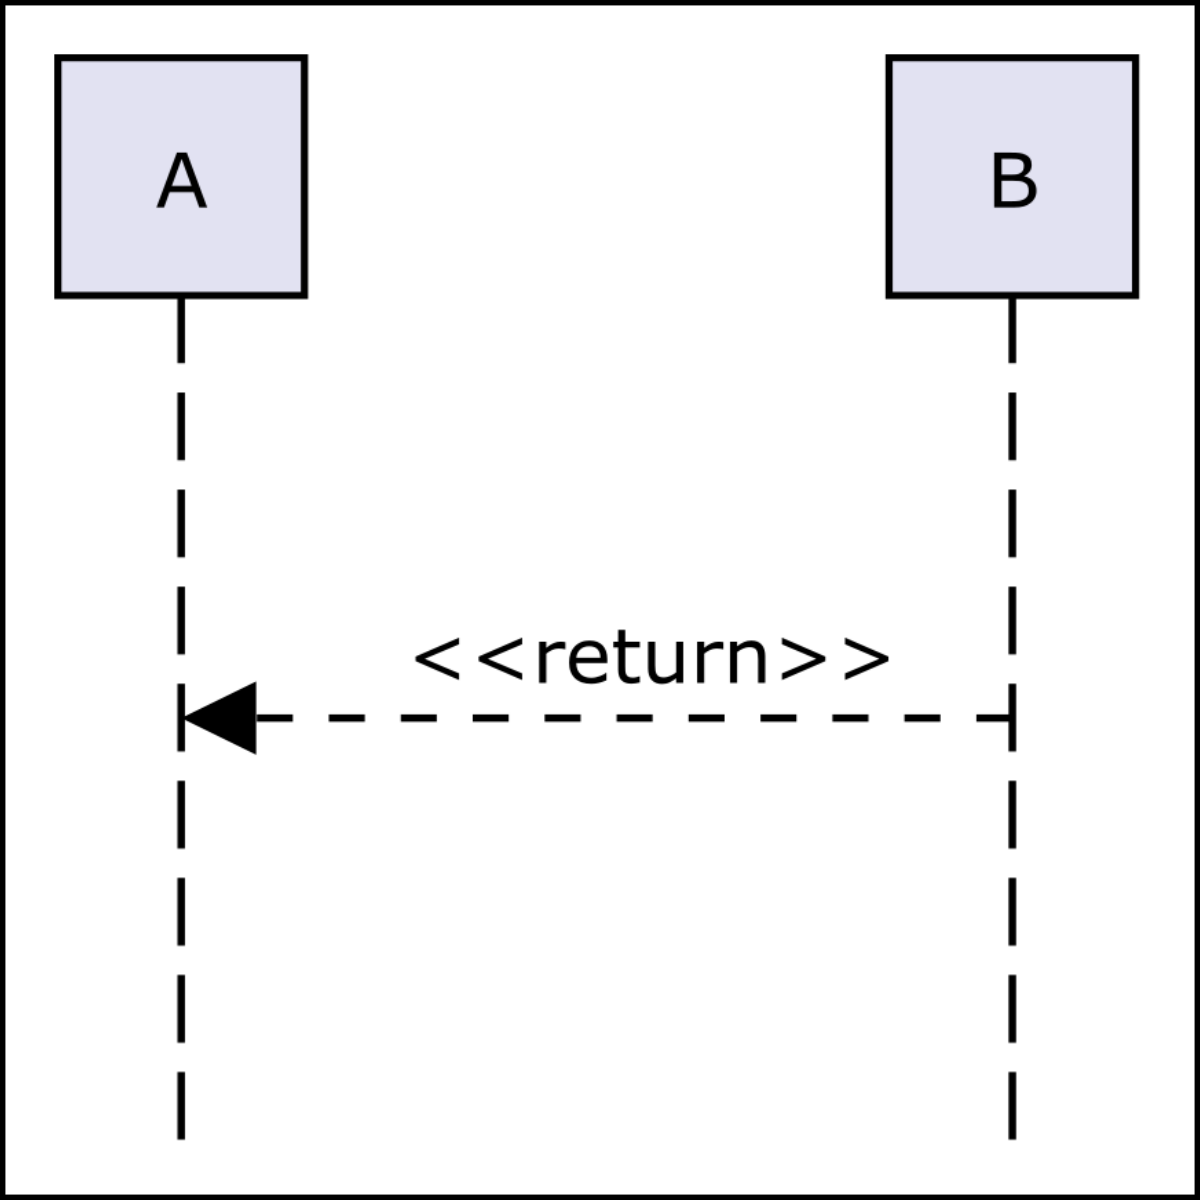
\includegraphics[width=0.25\textwidth]{Images/chapter_3/section_5224098311700480/5611954632916992.png}
 \caption{A synchronous return message}
\end{figure}

\begin{enumerate}
\setcounter{enumi}{3}
\item
A \textbf{create} \textbf{message} indicates that a new object is created during an interaction. New objects can be created as a result of some message or operation. We can draw it like this:
\end{enumerate}

\begin{figure}[htbp]
 \centering
 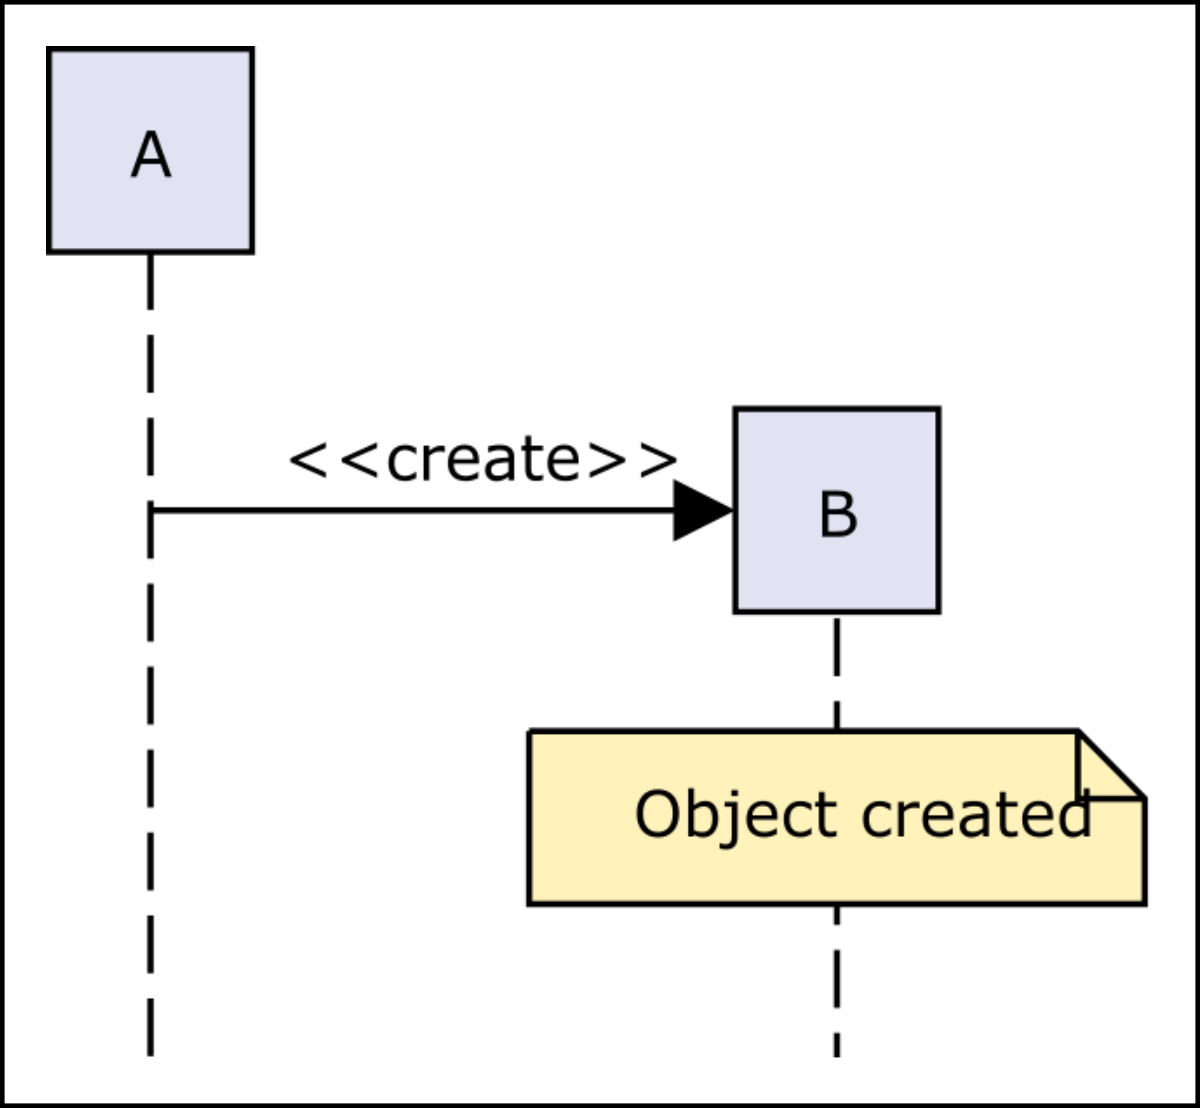
\includegraphics[width=0.25\textwidth]{Images/chapter_3/section_5224098311700480/4848348538601472.png}
 \caption{A create message}
\end{figure}

\begin{enumerate}
\setcounter{enumi}{4}
\item
A \textbf{destroy} \textbf{message} indicates that an object is destroyed during a sequence of events. Objects can be destroyed as a result of some message or operation, and their lifeline ends. We can draw it like this:
\end{enumerate}

\begin{figure}[htbp]
 \centering
 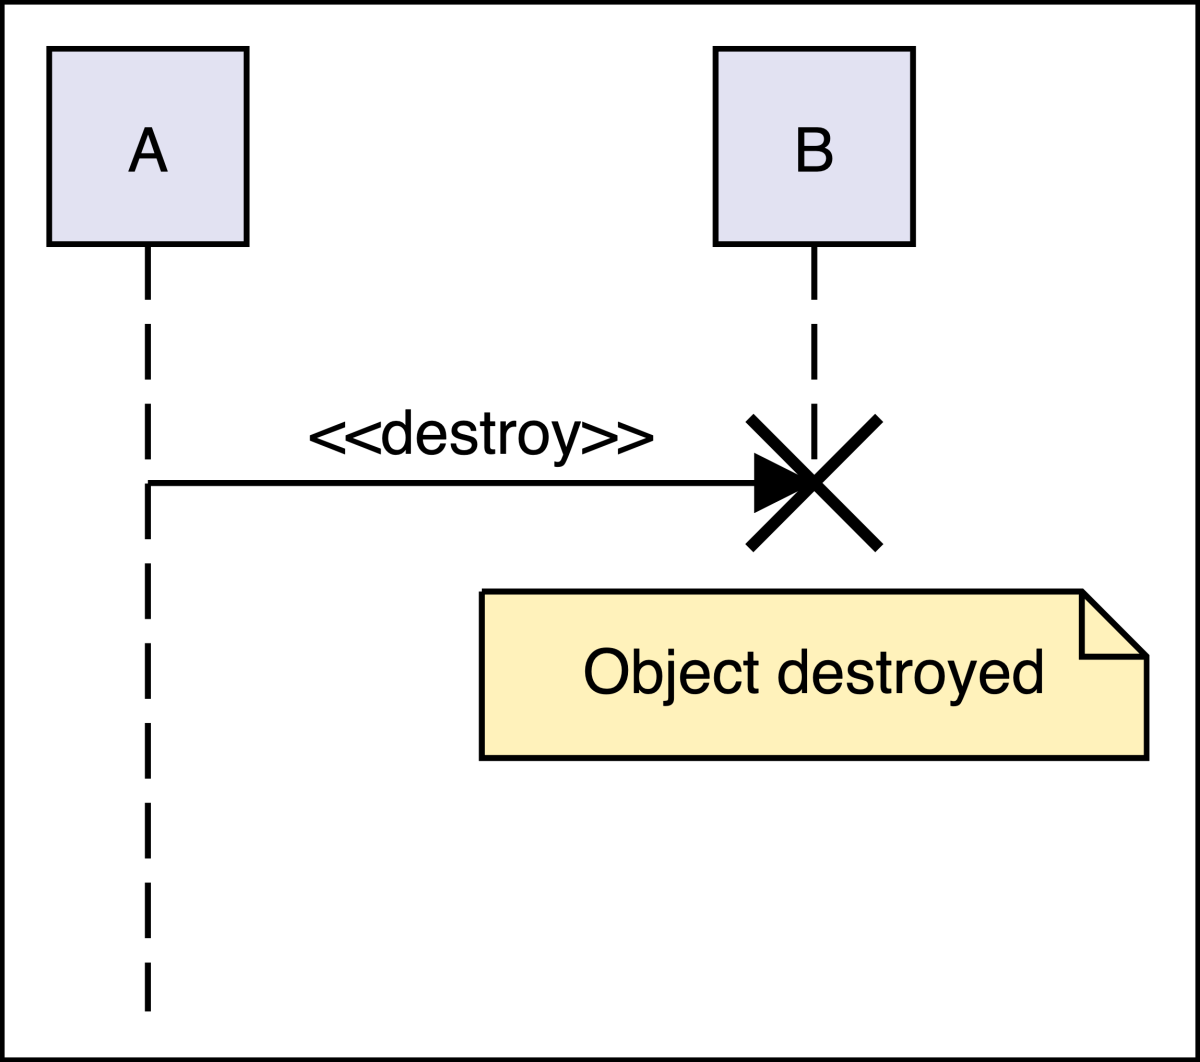
\includegraphics[width=0.25\textwidth]{Images/chapter_3/section_5224098311700480/5841913137856512.png}
 \caption{A destroy message}
\end{figure}

\begin{enumerate}
\setcounter{enumi}{5}
\item
A \textbf{lost message} is a message that initiates from an object but does not reach its endpoint. It appears as a message that is terminated. A \textbf{found message} is a message that is received, but the sender is unknown. It appears as a message that reaches an endpoint but does not initiate from any object. We draw lost messages as an arrow ending with a circle and found messages with an arrow starting with a circle.
\end{enumerate}

\begin{figure}[htbp]
 \centering
 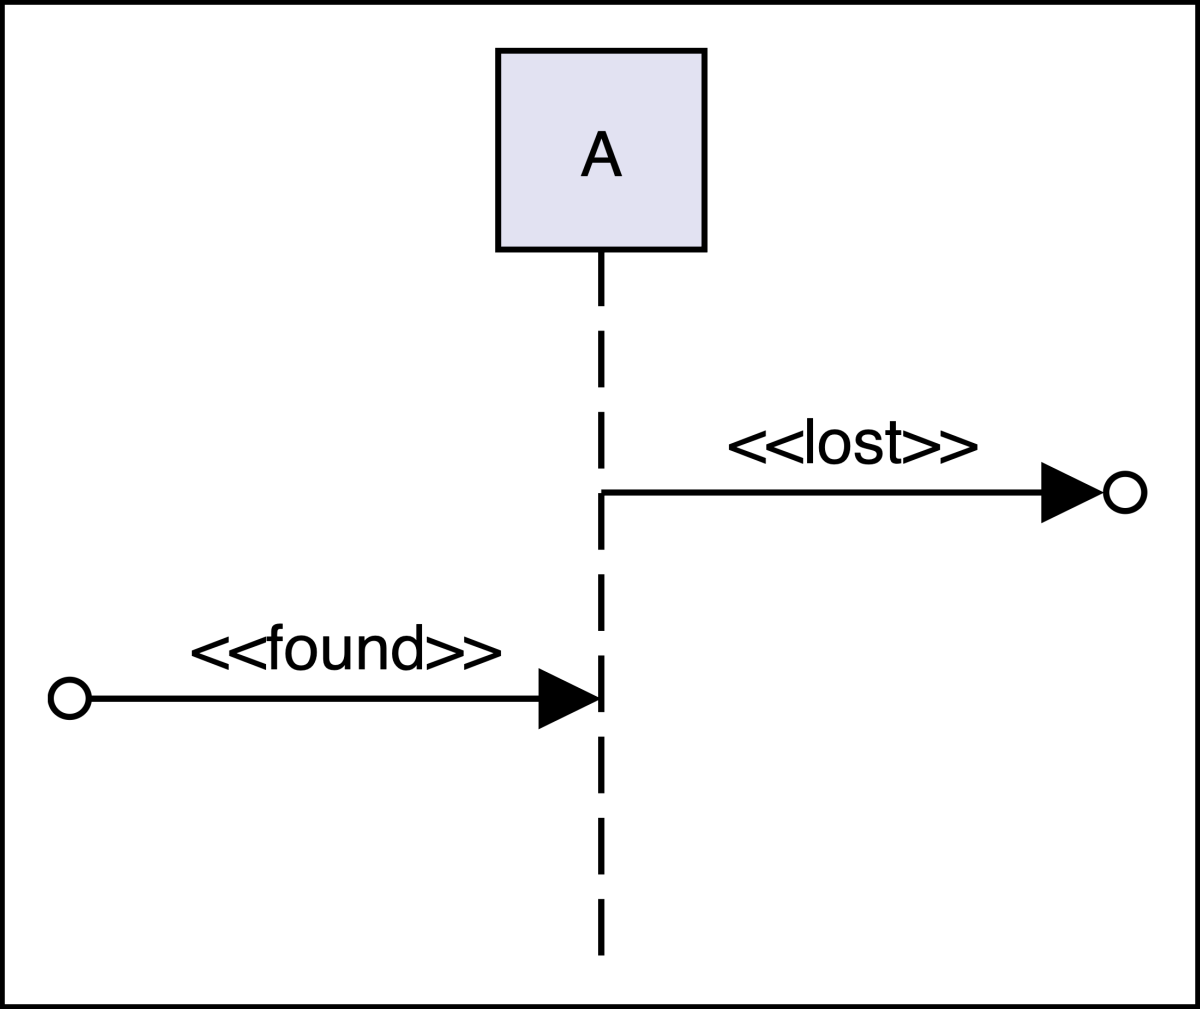
\includegraphics[width=0.25\textwidth]{Images/chapter_3/section_5224098311700480/5822636989087744.png}
 \caption{The lost and found messages}
\end{figure}

\begin{quote}
\textbf{Note:} Some sequence diagrams use filled circles to represent the lost and found messages. However, throughout the course we will apply the empty circle convention.
\end{quote}
\subsection{How to draw a sequence diagram}\label{how-to-draw-a-sequence-diagram}
\\
To create a self-explanatory sequence diagram, there are a number of steps that we need to follow. Before we start, it is important to understand that there isn\textquotesingle t one correct way of creating a sequence diagram. Some of us may have a different approach to handling these problems.
\\
In this lesson, we introduce a methodology that will help us break down the problem into smaller, achievable tasks. Let
\textquotesingle s take a look at the steps.

\subsubsection{Identify the use case}\label{identify-the-use-case}
\\
To get started with the sequence diagram, it is essential to know our use case. The sequence diagram is a means to define the sequential order of events that occur in that use case.
\\
Let\textquotesingle s build on a simple scenario where a customer wants to withdraw cash from an ATM. Our use case will be as follows:

\begin{figure}[htbp]
 \centering
 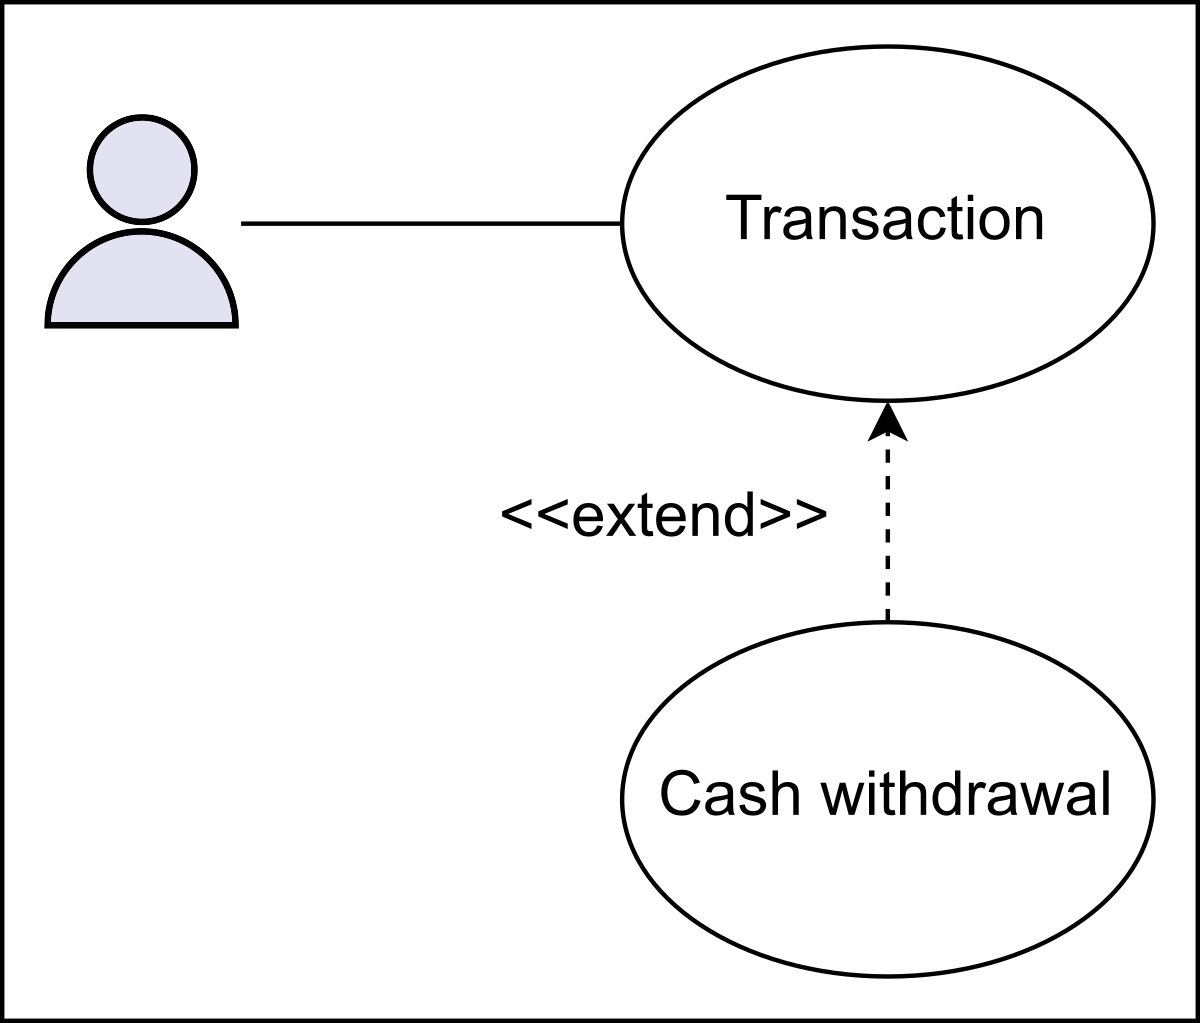
\includegraphics[width=0.25\textwidth]{Images/chapter_3/section_5224098311700480/5462020545839104.png}
 \caption{Use case for cash withdrawal}
\end{figure}

\subsubsection{Identify the actors and objects}\label{identify-the-actors-and-objects}
\\
Now, we need to list down all the actors and objects that will be involved in the entire sequence. These would be the following:

\begin{itemize}
\item
Customer
\item
ATM
\item
Transaction
\item
Account
\item
Cash dispenser
\end{itemize}

\subsubsection{Identify the order of actions}\label{identify-the-order-of-actions}
\\
We have identified the entities involved in the cash withdrawal sequence, but we don\textquotesingle t know how these entities will interact with each other. It is important that we note down the action and the order in which they will occur. Here
\textquotesingle s how we can define the interaction in steps:

\begin{enumerate}
\item
The customer requests a cash withdrawal from the ATM with their account information and the amount.
\item
The ATM initiates a cash withdrawal transaction against the account and the given amount.
\item
The transaction amount is verified for the given account.
\item
In case the amount entered is valid, the account verifies the transaction.
\item
The ATM signals the cash dispenser to release the required cash amount.
\item
The cash dispenser confirms the release of cash.
\item
The ATM prompts the user to collect the cash.
\end{enumerate}

\subsubsection{Create the diagram}\label{create-the-diagram}
\\
We have identified all the involved objects and entities in the interaction. We have also listed down the order in which the objects will perform these actions. To finally create the sequence diagram, we need to relate these steps with the type of messages that the objects will exchange with each other. Here
\textquotesingle s a possible diagram that we can create for the cash withdrawal scenario:

\begin{figure}[htbp]
 \centering
 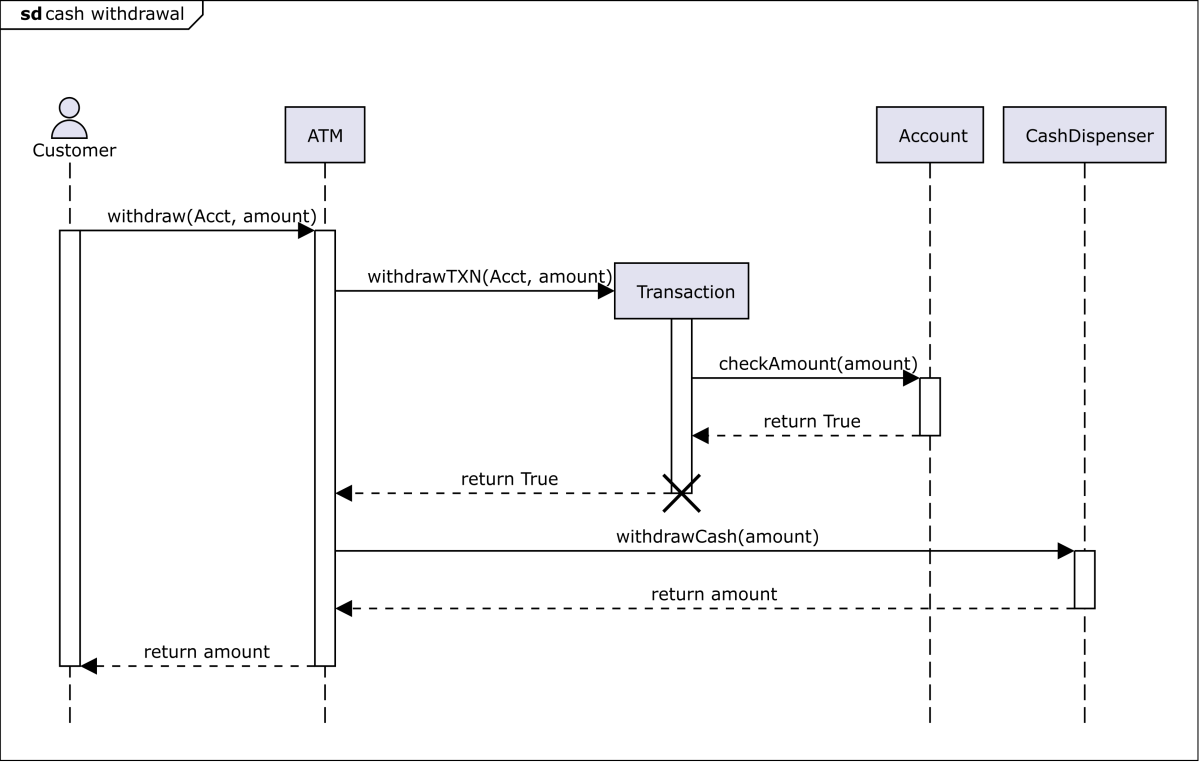
\includegraphics[width=0.5\textwidth]{Images/chapter_3/section_5224098311700480/6480178765365248.png}
 \caption{The sequence diagram for cash withdrawal}
\end{figure}

\subsection{Fragment frame in the sequence diagram}\label{fragment-frame-in-the-sequence-diagram}
\\
Our goal is to keep our sequence diagram as simple as possible without clutter and information overload. However, sometimes we need to show more complex actions like conditional actions or loop sequences. Sequence diagrams allow us to represent this information using the sequence fragment component. We can identify the operator of a fragment in the top left corner of the fragment frame. Here are a few examples of fragment operators:

\begin{itemize}
\item
\textbf{Alternative (alt):} This operator models the \texttt{if-else} condition. It divides the fragment into parts, and either of the parts can take place based on the guard condition.
\item
\textbf{Option (opt):} This operator models the \texttt{if} condition. The fragment will only execute if the guard condition is met. Otherwise, the entire fragment is skipped, and the interaction continues.
\item
\textbf{Loop (loop):} This operator represents a repetitive sequence. The fragment will keep repeating until the guard condition is met.
\item
\textbf{Reference (ref):} This operator assists in managing larger diagrams. It allows us to reuse parts of another sequence diagram by providing a reference to it.
\end{itemize}
\\
Let\textquotesingle s expand the sequence diagram we created to see how we can build on it further using a sequence fragment.

\begin{figure}[htbp]
 \centering
 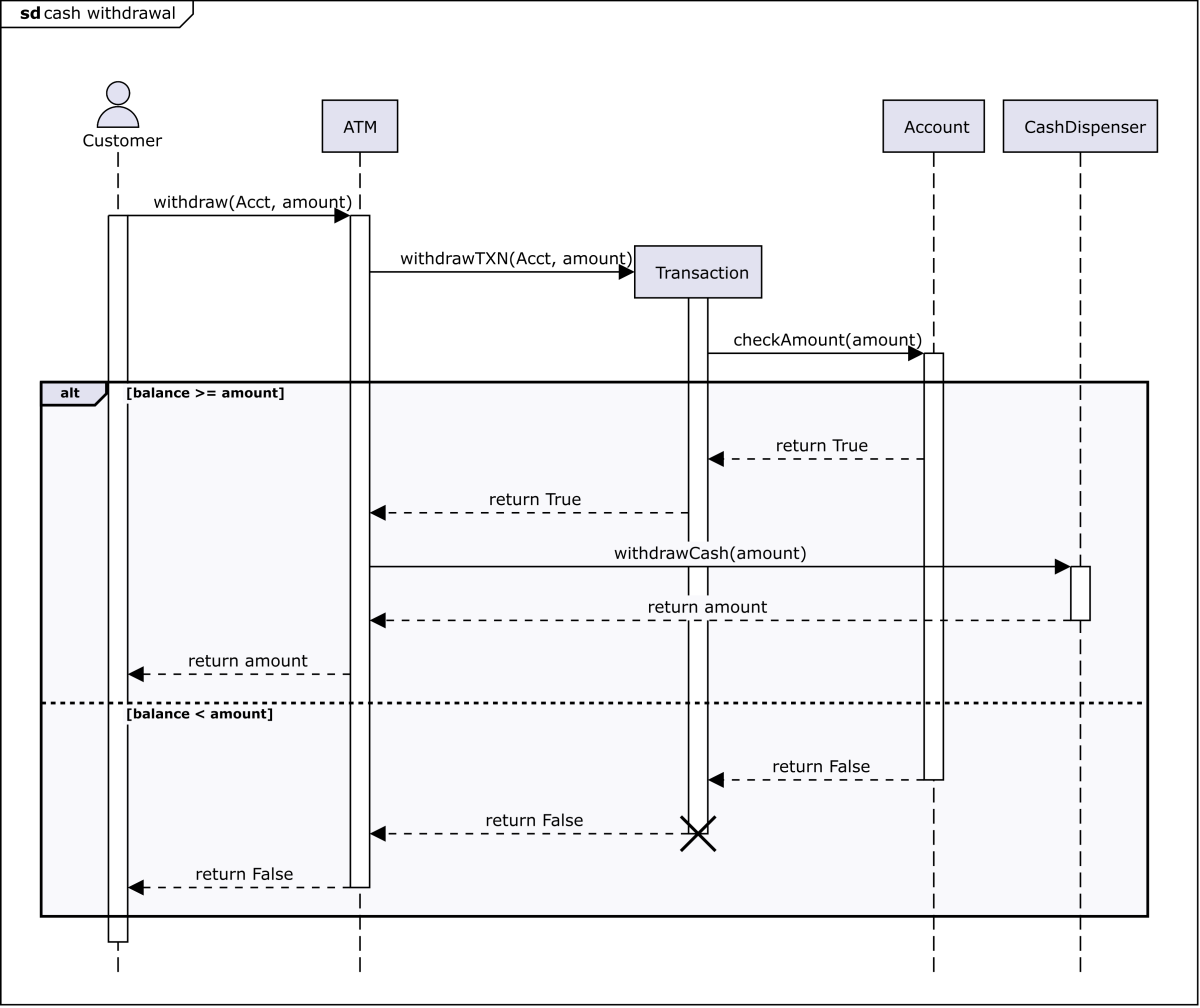
\includegraphics[width=0.5\textwidth]{Images/chapter_3/section_5224098311700480/6020048729931776.png}
 \caption{The sequence diagram for cash withdrawal with a sequence fragment}
\end{figure}

In the diagram above, we add the alternatives operator, which divides the sequence into two fragments. The first fragment takes place if the guard condition is met, while in any other case, the second fragment occurs. Here the guard condition is that the balance in the account should be greater than or equal to the amount requested by the customer.
\\
Next, let\textquotesingle s look at the different elements of an activity diagram and how to construct it.

\subsection{}\label{section}

% End of section content